\documentclass[11pt]{article}

\usepackage[utf8]{inputenc}
\usepackage[spanish]{babel}
\usepackage{graphicx}
\usepackage{physics}
\usepackage{amssymb}
\usepackage{enumerate}

\usepackage{authblk}

\title{Simetría: Partículas como representaciones del grupo de Poincaré}
\author{Iván Mauricio Burbano Aldana}
\affil{Universidad de los Andes}

\DeclareMathOperator{\Gl}{GL}
\DeclareMathOperator{\Sl}{SL}
\DeclareMathOperator{\SU}{SU}
\DeclareMathOperator{\SO}{SO}
\DeclareMathOperator{\id}{id}

\begin{document}

\maketitle

\begin{abstract}
El desarrollo de la relatividad especial aclaró la estructura espaciotemporal sobre la cual se ha formulado el modelo estándar de partículas. En particular, resalta un conjunto de transformaciones, el grupo de Poincaré, que preserva esta estructura. Sorprendentemente, el requerimiento natural de que el conjunto de estados de un sistema cuántico sea un espacio de representación de este grupo, lleva de manera natural al concepto de partícula como representación irreducible etiquetada con masa y espín\cite{Wigner1939}. Ya que este requerimiento se puede extender a otros grupos de simetrías (internas), responsables de la diversidad de partículas en el modelo estandar, el ejemplo relativista forma un punto de partida importante para ejemplificar la interacción entre simetría y partículas. Después de caracterizar el grupo de Poincaré siguiendo \cite{Scheck2010}, seguiremos el camino de ``físicos''\cite{Haag1992}\cite{Weinberg1995} para mostrar como el concepto de partícula surge de la invariancia de Lorentz. Sin embargo, se hará un esfuerzo por notar las partes no rigurosas de los argumentos estándar y, bajo la tutoría de \cite{Straumann2008}, indicar los caminos a solucionarlas.  
\end{abstract}

\section{Transformaciones de Lorentz}

Empecemos realizando un breve recuento de las transformaciones de Lorentz. Si bien principalmente seguiremos la exposición en \cite{Scheck2010}, una versión más formal (y bella debido a su independencia explicita de sistemas de referencia) se encuentra en \cite{Matolcsi1993}.

El espaciotiempo relativista (especial) se conforma de la siguiente estructura de datos $(M,g)$ donde $M$ es un espacio afín real de cuatro dimensiones sobre un espacio vectorial $\vb{M}$ y $g:\vb{M}\cross\vb{M}\rightarrow I\otimes I$ una forma de Lorentz. Como se muestra en \cite{Matolcsi1993} cada espaciotiempo relativista es isomorfo al modelo aritmético $(\mathbb{R}^4,\eta)$ donde\footnote{A lo largo de este documento utilizaremos la convención de suma de Einstein. Los indices latinos irán a lo largo de $\{0,1,2,3,4\}$ mientras que los griegos de $\{1,2,3\}$. Además escogemos unidades donde la velocidad de la luz $c=1$.}
\begin{align}
\begin{split}
\eta:\mathbb{R}^4\times\mathbb{R}^4&\rightarrow\mathbb{R} \\
(u,v)&\mapsto \eta_{ab}u^a v^b
\end{split}
\end{align}  
y 
\begin{equation}
\eta_{ab}=\mqty[1 & 0 & 0 & 0 \\ 0 & -1 & 0 & 0 \\ 0 & 0 & -1 & 0 \\ 0 & 0 & 0 & -1]_{ab}
\end{equation}
Note que si bien a nivel estructural el modelo aritmético es el único modelo de espaciotiempo relativista salvo isomorfismo, no hay ninguna razón por la cual escogerlo sobre los otros. En este trabajo lo haremos debido a nuestra familiaridad con los objetos involucrados en este. Sin embargo es importante hacer la salvedad: ¡No hemos escogido un sistema de referencia! En particular es importante distinguir entre los puntos del espaciotiempo $\mathbb{R}^4$ y los vectores (translaciones entre puntos) en el espacio modelo $\mathbb{R}^4$. En particular, el punto $(0,0,0,0)$ no tiene nada de especial con respecto a los otros puntos mientras que el vector $(0,0,0,0)$ sí. Por otra parte, las componentes de un vector $u\in\mathbb{R}^4$ no son las componentes medidas por ningún observador. Para poder definir estas es necesario incluir un sistema de referencia lo cual induce una partición del espaciotiempo. Para más discusión ver \cite{Matolcsi1993}.

Ahora estudiemos los mapas que preservan estructura entre espaciotiempos aritméticos. Estos son los mapas afines (debido a la estructura afín de estos modelos)
\begin{align}
\begin{split}
\mathbb{R}^4\rtimes \Gl(\mathbb{R}^4)\ni(a,\Lambda):\mathbb{R}^4&\rightarrow\mathbb{R}^4 \\
p&\mapsto\Lambda p + a
\end{split}
\end{align}
que preservan la forma de Lorentz
\begin{equation}
\eta(u,v)=\eta(\Lambda u,\Lambda v)
\end{equation}
La estructura de producto semidirecto es clara de la regla de composición que queremos que se cumpla
\begin{equation}
(u,\Lambda)(u',\Lambda')p=(u,\Lambda)(\Lambda 'p+u')=\Lambda(\Lambda 'p+u')+u=(\Lambda u'+u,\Lambda\Lambda ')p
\end{equation} 
Así mismo se puede verificar que estos mapas forman un subgrupo de $\mathbb{R}^4\rtimes\Gl(\mathbb{R}^4)$ al cual llamamos el grupo de Poincaré $\mathcal{P}$. Los elementos $\Lambda\in\Gl(\mathbb{R}^4)$ tal que $(\Lambda,0)\in\mathcal{P}$ forman un subgrupo de $\Gl(\mathbb{R}^4)$ conocido como el grupo de Lorentz $\mathcal{L}$. Podemos identificar cuatro subconjuntos $\mathcal{L}_+^\uparrow$, $\mathcal{L}_+^\downarrow$, $\mathcal{L}_-^\uparrow$ y $\mathcal{L}_-^\downarrow$ de $\mathcal{L}$ donde el signo $\pm$ determina si $\det\Lambda=\pm 1$ y la flecha determina si $\Lambda^0_0\geq 1$ ($\uparrow$) o $\Lambda^0_0\leq -1$ ($\downarrow$). Estas resultan ser las cuatro componentes conexas de $\mathcal{L}$ y se tienen las siguientes conexiones entre ellas: $\mathcal{L}_-^\uparrow=P\mathcal{L}_+^\uparrow$, $\mathcal{L}_-^\downarrow=T\mathcal{L}_+^\uparrow$ y $\mathcal{L}_+^\downarrow=PT\mathcal{L}_+^\uparrow$ donde $P$ es la transformación de paridad
\begin{align}
\begin{split}
P:\mathbb{R}^4&\rightarrow\mathbb{R}^4 \\
(v^0,v^1,v^2,v^3)&\mapsto(v^0,-v^1,-v^2,-v^3)
\end{split}
\end{align}
y $T$ la de inversión temporal $T=-P$. Debido a estas formulas y a nuestro objetivo de describir el surgimiento de masa y espín solo nos enfocaremos en la descripción del grupo de Lorentz ortocrono propio $\mathcal{L}_+^\uparrow$ y su grupo de Poincaré asociado $\mathcal{P}_+^\uparrow=\mathbb{R}^4\rtimes\mathcal{L}_+^\uparrow$.

Como veremos en la siguiente sección, es importante estudiar la relación entre el grupo $\Sl(\mathbb{C}^2)$ de operadores invertibles de determinante 1 sobre $\mathbb{C}^2$ y $\mathcal{P}_+^\uparrow$. En primer lugar note el ismorfismo
\begin{align}
\begin{split}
\Phi:\mathbb{R}^4&\rightarrow\{A:\mathbb{C}^2\rightarrow\mathbb{C}^2|\text{$A$ es autoadjunta}\} \\
(v^0,v^1,v^2,v^3)&\mapsto\mqty[v^0+v^3 & v^1-iv^2 \\ v^1 + iv^2 & v^0-v^3]=v^a\sigma_a. 
\end{split}
\end{align}
Su importancia recae en que
\begin{equation}
\eta(v,v)=\det(\Phi(v)).
\end{equation}
Por lo tanto la transformación $A\mapsto\alpha A\alpha^*$ al preservar determinantes para toda $\alpha\in\Sl(\mathbb{C}^2)$ puede verse como una transformación de Lorentz
\begin{align}
\begin{split}
\Lambda:\Sl(\mathbb{C}^2)\rightarrow\mathcal{L}_+^\uparrow \quad & \\
\alpha\mapsto \Lambda(\alpha):\mathbb{R}^4&\rightarrow\mathbb{R}^4 \\
 v & \mapsto\Phi^{-1}(\alpha\Phi(v)\alpha^*)
\end{split}
\end{align}
Note que $\mathcal{L}_+^\uparrow$ no es simplemente conexo. En efecto una rotación por $2\pi$ es un lazo que no puede ser deformado continuamente a la identidad. Sin embargo, $\Sl(\mathbb{C}^2)$ sí lo es y es el recubridor universal de $\mathcal{L}_+^\uparrow$. Así mismo, $\mathbb{R}^4\rtimes\Sl(\mathbb{C}^2)$ es el de $\mathcal{P}_+^\uparrow$. Si bien no hay momento para discutirlo en este lugar, esta conexión y las representaciones de $\Sl(\mathbb{C}^2)$ sobre espacios complejos de dimensión finita dan lugar a el concepto de espinores y son suficientes para deducir la ecuación de Klein-Gordon, Dirac, y sus generalizaciones para espines más altos\cite{Haag1992}.

\section{Grupos de simetría en mecánica cuántica}

Habiendo identificado $\mathcal{L}_+^\uparrow$ como un grupo de simetrías fundamentales de la física, ahora pasemos a entender de manera general la interacción entre grupos de simetrías y mecánica cuántica. Para esto extenderemos la discusión dada en \cite{Haag1992}.

Suponga que un sistema cuántico está descrito por un espacio de Hilbert $\mathcal{H}$. Los estados puros entonces son las proyecciones ortogonales $\rho_\psi$ sobre el subespacio generado por $\psi\in\mathcal{H}$. Es claro que un estado puro $\rho_\psi$ puede ser entendido como una proposición que corresponde a la observación ``el sistema está en el estado $\rho_\psi$''. Por lo tanto, si el sistema se encuentra en el estado puro $\rho_\phi$, la probabilidad de obtener el estado $\rho_\psi$ luego de una medición de este observable es
\begin{equation}
\tr(\rho_\psi\rho_\phi)=\frac{\langle\phi,\rho_\psi\phi\rangle}{\langle\phi,\phi\rangle}=\frac{\langle\phi,\langle\psi,\phi\rangle\psi\rangle}{\langle \phi,\phi\rangle\langle\psi,\psi\rangle}=\frac{|\langle\phi,\psi\rangle|^2}{\|\phi\|^2\|\psi\|^2}.
\end{equation}

Si $G$ es un grupo de simetrías del sistema, se debe inducir un mapa $T$ que a cada $g\in G$ asigna una transformación de estados puros $T(g)$ que preserva estos productos internos, es decir
\begin{equation}
\tr(T(g)(\rho_\psi)T(g)(\rho_\phi))=\tr(\rho_\psi\rho_\phi),
\end{equation} 
y respeta la ley de grupo $T(g)\circ T(g')=T(gg')$. Debido a la interpretación de estas trazas, es exactamente la existencia de tal mapa la que hace que $G$ sea un grupo de simetrías del sistema. Sin embargo, estos mapas de estados son difíciles de manejar y nos gustaría trabajar con mapas entre vectores. Resulta que una transformación de estados puros como la anterior se puede siempre reemplazar por una de vectores lineal y unitaria o antilineal y antiunitaria que queda completamente determinada excepto por una fase\cite{Haag1992}. Este último caso no es posible cuando trabajamos con grupos continuos. Concluimos entonces que si $G$ es continuo, a cada $g\in G$ le corresponde un operador unitario $U(g)$ sobre $\mathcal{H}$ de manera que $U(g)U(g')=\chi(g,g')U(gg')$ donde $\chi(g,g')$ es una fase. Resulta que para el grupo $\mathcal{P}_+^\uparrow$ podemos tomar la fase $\chi(g,g')=1$ si consideramos el grupo de simetrías como su recubridor universal $\mathbb{R}^4\rtimes\Sl(\mathbb{C}^2)$\cite{Haag1992}. 

Concluimos entonces que: si el grupo ortocrono propio de Poincaré es un grupo de simetrías de la física entonces toda teoría descrita en un espacio de Hilbert $\mathcal{H}$ debe llevar una representación unitaria de $\mathbb{R}^4\rtimes\Sl(\mathbb{C}^2)$, es decir, un homomorfismo $U:\mathbb{R}^4\rtimes\Sl(\mathbb{C}^2)\rightarrow U(\mathcal{H})$ donde $U(\mathcal{H})$ es el grupo de transformaciones unitarias de $\mathcal{H}$.

\section{Representaciones irreducibles del grupo de Poincaré}

Habiendo descrito el grupo de Poincaré ortocrono propio y su recubridor universal, estamos listos para discutir la teoría de representaciones asociada siguiendo a Haag\cite{Haag1992}. El primer paso es notar que al tener representaciones unitarias, existen operadores $P_a$ autoadjuntos tal que
\begin{equation}
U(a,\id_{\mathbb{C}^2})=e^{iP_b a^b}.
\end{equation}
Es de notar que tal exponencial se define mediante la teoría espectral de los operadores $P_a$. Como el subgrupo de traslaciones es abeliano, se tiene por la fórmula de Baker-Campbell-Hausdorff que los $P_a$ conmutan. Ahora bien, para $\epsilon\in\mathbb{R}^4$ infinitesimal
\begin{align}
\begin{split}
\id_\mathcal{H} + i\epsilon^a U(0,\alpha)^{-1}P_a U(0,\alpha) &=U(0,\alpha)^{-1}(\id_\mathcal{H}+iP_a \epsilon^a)U(0,\alpha) \\
&=U(0,\alpha)^{-1}U(\epsilon,\id_{\mathbb{C}^2})U(0,\alpha) \\
&= U((0,\alpha^{-1})(\epsilon,\id_{\mathbb{C}^2})(0,\alpha)) \\
&=U((\Lambda(\alpha^{-1})\epsilon,\alpha^{-1})(0,\alpha)) \\
&=U((\Lambda(\alpha)^{-1} \epsilon, \id_{\mathbb{C}^2})) \\
&=\id_\mathcal{H}+i(\Lambda(\alpha)^{-1})^a_b\epsilon^b P_a.
\end{split}
\end{align}
Se concluye entonces que
\begin{equation}\label{eq:momento}
U(0,\alpha)^{-1}P^a U(0,\alpha) = \Lambda(\alpha)^a_b P^b
\end{equation}
El hecho de que conmutan, generan traslaciones y transforman como vectores, nos invita a interpretar los operadores $P^a$ como los de energía-momento. Como conmutan, tienen una resolución espectral simultanea y podemos construir los espacios $\mathcal{H}_p$ de momento definido $p\in\mathbb{R}^4$. Esto significa que si $\psi\in\mathcal{H}_p$ se tiene que $P^a\psi=p^a \psi$. Note que estos espacios no son subespacios de $\mathcal{H}$ si el espectro de $P^a$ es continuo. Esto sucede también en teorías no relativistas y por lo tanto los trataremos como si lo fueran. Más aún, \eqref{eq:momento} muestra que $U(0,\alpha)$ lleva a $\mathcal{H}_p$ hasta $\mathcal{H}_{\Lambda(\alpha)p}$. Una representación irreducible es aquella donde los únicos subespacios invariantes son triviales, es decir, $\{0\}$ y $\mathcal{H}$. Luego, si $U$ es irreducible, los espacios $\mathcal{H}_p$ que aparecen en la representación estarán etiquetados por $\{\Lambda(\alpha)p\in\mathbb{R}^4|\alpha\in\Sl(\mathbb{C}^2)\}$ la órbita de $p$. En efecto si aparecen más momentos, el espacio antes descrito va a ser un subespacio invariante no trivial y si aparecen menos, vamos a poder salirnos del dominio mediante acción del grupo de Poincaré ortocrono propio y no vamos a obtener una representación. Esto nos lleva a una primera clasificación de los irreducibles:
\begin{center}
\begin{tabular}{|c|c|}
\hline
clase & órbita \\
\hline
$m_+$ & $\eta(p,p)=m^2$ y $p^0>0$ \\
$0_+$ & $\eta(p,p)=0$ y $p^0\geq 0 $ \\
$0_0$ & $p=0$ \\
$\kappa$ & $\eta(p,p)=-\kappa^2$ \\
$m_-$ & $\eta(p,p)=m^2$ y $p^0<0$ \\
$0_-$ & $\eta(p,p)=0$ y $p^0\leq 0$ \\
\hline
\end{tabular}
\end{center}
Entre estas, solo las clases $m_+$ y $0_+$ han sido observadas. Por otra parte, la clase $0_0$ sirve como una descripción del vacío. Por la interpretación de $P^a$ tenemos que $m=\sqrt{\eta(p,p)}$ toma la interpretación de masa en reposo. Para finalizar el análisis, tome un momento $\overline{p}$ en cada órbita y defina $\beta(p)\in\Sl(\mathbb{C}^2)$ tal que $\Lambda(\beta(p))\overline{p}=p$. La teoría generar de representaciones de grupo nos indica que las representaciones del subgrupo que deja invariante a $\overline{p}$ son las irreducibles para cada órbita $\overline{p}$. 

\begin{figure}
\centering
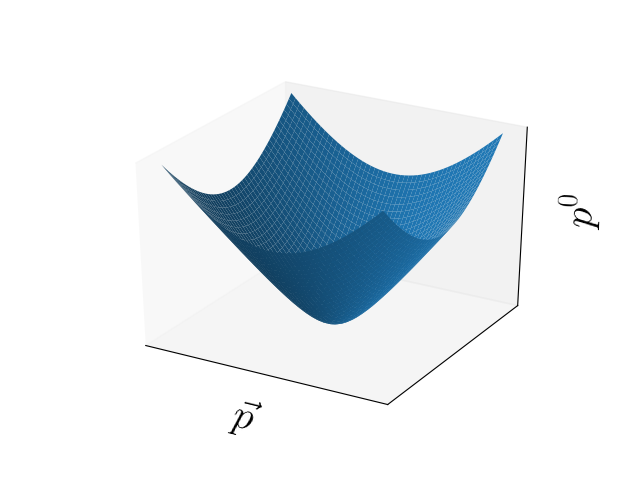
\includegraphics[width=0.7\textwidth]{hiperboloide.png}
\caption{Se muestra una órbita de clase $m_+$}
\end{figure}

Ahora considere una representación en la clase $m_+$. Un espacio que aparecerá en tal representación es $\mathcal{H}_{\overline{p}}$ con $\overline{p}=(m,0,0,0)$. Si $p\in\mathbb{R}^4$ es tal que $\eta(p,p)=m^2$ y $p^0>0$ tome 
\begin{equation}
\beta(p)=\left(\frac{E_p\id_{\mathbb{C}^2}+\sum_{\mu=1}^3p^\mu\sigma_\mu}{m}\right)^{1/2}
\end{equation}
con $E_p=\sqrt{\sum_{\mu=1}^3(p^\mu)^2+m^2}=p^0$. Entonces
\begin{align}
\begin{split}
\Lambda(\beta(p))\overline{p}&=\Phi^{-1}(\beta(p)\Phi(\overline{p})\beta(p)^*) \\
&=\Phi^{-1}\left(\left(\frac{E_p\id_{\mathbb{C}^2}+\sum_{\mu=1}^3p^\mu\sigma_\mu}{m}\right)^{1/2}m\left(\left(\frac{E_p\id_{\mathbb{C}^2}+\sum_{\mu=1}^3p^\mu\sigma_\mu}{m}\right)^{1/2}\right)^*\right) \\
& = \Phi^{-1}\left(\left(E_p\id_{\mathbb{C}^2}+\sum_{\mu=1}^3p^\mu\sigma_\mu\right)^{1/2}\left(E_p\id_{\mathbb{C}^2}+\sum_{\mu=1}^3p^\mu\sigma_\mu\right)^{1/2}\right) \\
& = \Phi^{-1}\left(E_p\sigma_0 + \sum_{\mu=1}^3p^\mu\sigma_\mu\right) = (E_p, p^1, p^2, p^3) = p.
\end{split}
\end{align}

Ahora bien, note que el grupo de isotropía, es decir, el subgrupo de $\Sl(\mathbb{C}^2)$ que deja a $\overline{p}$ invariante satisface que
\begin{equation}
\overline{p} = \Lambda(\alpha)(\overline{p}) = \Phi^{-1}(\alpha\Phi(\overline{p})\alpha^*) = \Phi^{-1}(m\alpha\alpha^*)=m\Phi^{-1}(\alpha\alpha^*).
\end{equation} 
Concluimos que el grupo de isotropía es $\SU(\mathbb{C}^2)$ el recubridor universal de $\SO(\mathbb{R}^3)$. La teoría de representaciones de este grupo es bien conocida ya que aparece en el estudio de momento angular en mecánica cuántica no relativista. Estas están etiquetadas por una etiqueta de espín $s\in\mathbb{N}/2$. Con esto se obtienen representaciones irreducibles de $\Sl(\mathbb{C}^2)$ con masa $m>0$ y espín $s$. 

El caso $0_+$ es similar. Sin embargo, el grupo de isotropía va a tener representaciones etiquetadas por $s\in\mathbb{Z}/2$ conocido como helicidad.

\section{Conclusiones y comentarios finales}

Despues de describir en detalle los grupos de simetría del espaciotiempo relativista y la necesidad de tener representaciones de el en cualquier teoría cuántica, llegamos a que las representaciones irreducibles estaba determinadas por etiquetas de masa $m$ y espín (o helicidad) $s$. Para esto se llevo a cabo el siguiente programa\cite{Sternberg1994}:
\begin{enumerate}[(i)]
\item Encontrar las órbitas de $\Sl(\mathbb{C}^2)$.
\item Escoger un punto en la órbita y hallar su grupo de isotropía.
\item Encontrar las representaciones irreducibles de este.
\end{enumerate}

Encontramos entonces una manera matemáticamente rigurosa de clasificar partículas. Esta se puede extender teniendo en cuenta otros grupos de simetrías internas. En particular, esta no depende de la noción de campos. Esto es importante ya que se puede obtener la misma teoría escogiendo distintos campos. Por esto el estudio de la teoría algebráica cuántica de campos promete ser una manera de solucionar los problemas de consistencia interna de las teorías modernas al proveer una representación más exacta y directa de la realidad física\cite{Haag1992}.

\bibliography{/home/ivan/Documents/Bib_Files/particle_physics_2017_II}
\bibliographystyle{ieeetr}

\end{document}
